%%
%% This is file `sample-sigplan.tex',
%% generated with the docstrip utility.
%%
%% The original source files were:
%%
%% samples.dtx  (with options: `all,proceedings,bibtex,sigplan')
%% 
%% IMPORTANT NOTICE:
%% 
%% For the copyright see the source file.
%% 
%% Any modified versions of this file must be renamed
%% with new filenames distinct from sample-sigplan.tex.
%% 
%% For distribution of the original source see the terms
%% for copying and modification in the file samples.dtx.
%% 
%% This generated file may be distributed as long as the
%% original source files, as listed above, are part of the
%% same distribution. (The sources need not necessarily be
%% in the same archive or directory.)
%%
%%
%% Commands for TeXCount
%TC:macro \cite [option:text,text]
%TC:macro \citep [option:text,text]
%TC:macro \citet [option:text,text]
%TC:envir table 0 1
%TC:envir table* 0 1
%TC:envir tabular [ignore] word
%TC:envir displaymath 0 word
%TC:envir math 0 word
%TC:envir comment 0 0
%%
%%
%% The first command in your LaTeX source must be the \documentclass
%% command.
%%
%% For submission and review of your manuscript please change the
%% command to \documentclass[manuscript, screen, review]{acmart}.
%%
%% When submitting camera ready or to TAPS, please change the command
%% to \documentclass[sigconf]{acmart} or whichever template is required
%% for your publication.
%%
%%
\documentclass[sigplan,screen]{acmart}


\begin{document}

%%
%% The "title" command has an optional parameter,
%% allowing the author to define a "short title" to be used in page headers.
\title{A Comparative Study of the Generative Textual Data and Organic Textual Data}
\subtitle{INFO 5731 - Computational Methods for Information Systems\\
Section - 020\\Spring 2024
}

%%
%% The "author" command and its associated commands are used to define
%% the authors and their affiliations.
%% Of note is the shared affiliation of the first two authors, and the
%% "authornote" and "authornotemark" commands
%% used to denote shared contribution to the research.
\author{Mike Chastain}
\affiliation{%
  \institution{University of North Texas}
  \streetaddress{} % Added empty streetaddress to prevent error
  \studentid{}
  \city{}
  \state{}
  \country{}
}

\author{Harish Babu Kancharla}
\affiliation{%
  \institution{University of North Texas}
  \streetaddress{}
  \studentid{}
  \city{}
  \state{}
  \country{}
}

\author{Gnaneswara Reddy Palem}
\affiliation{%
  \institution{University of North Texas}
  \streetaddress{}
  \studentid{}
  \city{}
  \state{}
  \country{}
}

\author{Sai Sampath Varma Byrraju}
\affiliation{%
  \institution{University of North Texas}
  \streetaddress{}
  \studentid{}
  \city{}
  \state{}
  \country{}
}

\author{Sireesha Rusum}
\affiliation{%
  \institution{University of North Texas}
  \streetaddress{}
  \studentid{}
  \city{}
  \state{}
  \country{}
}

\author{Sri Naga Tejaswini Gandikota}
\affiliation{%
  \institution{University of North Texas}
  \streetaddress{}
  \studentid{}
  \city{}
  \state{}
  \country{}
}


%%
%% By default, the full list of authors will be used in the page
%% headers. Often, this list is too long, and will overlap
%% other information printed in the page headers. This command allows
%% the author to define a more concise list
%% of authors' names for this purpose.
\renewcommand{\shortauthors}{}




\maketitle
\section{Abstract}

This study shows the comparison between organic data and the synthetic data with the help of analytic techniques: text summarization in journalism domain and side-effect extraction in medical domain. This study intends to assess the influence of these data kinds on downstream task performance and knowledge development by utilizing statistical analysis, including metrics like mean and standard deviation. This process entails gathering organic data from trustworthy human-driven sources and creating synthetic data with cutting-edge AI tools. For the two jobs, the datasets undergo preprocessing and similar procedures. Models are trained to recognize and extract negative medical outcomes from textual data in the side effect extraction challenge. The ability of models to provide succinct, insightful summaries is examined in the text summarization task. A comparative analysis of the statistical properties of the two data formats and their impact on task accuracy, precision, and recall will be part of the study's findings. In addition to providing insights into potential biases or restrictions, the results should reveal significant differences in the learning behaviors of models trained on synthetic versus organic data. To improve the integration of synthetic data into practical applications, the study also suggests mitigating measures to solve issues that have been found. This study advances knowledge of the practical applications of generative AI tools in the medical and more general NLP domains, as well as their dependability.

The code, data, analysis, and results can be accessed on GitHub at: \url{https://github.com/180030814-GnaneshwarReddy/INFO-Group-9/tree/main}

\section{Keywords}
Named Entity Recognition(NER), Generative Artificial Intelligence(GAI), BioBERT, Pegasus-XSum, BART-Large-CNN, T5-small, Standard deviation, SIDER Database, Synthetic Data Generation, MedDRA Dictionary, Precision, Recall, F1 Score, Completeness, Consistency, Representativeness.

\section{Introduction}

The six students of INFO 5731 Group 9 aim to compare human-generated (organic) textual data with generative artificial intelligence (GAI) sources to explore the potential of GAI in creating synthetic data for training and testing models. The group task organized itself by splitting into two sub-groups to focus on two tasks: side effect extraction, using Named Entity Recognition (NER), and Text Summarization. This study is significant because it addresses challenges such as data scarcity, privacy concerns, and class imbalance, which are prevalent in critical domains like healthcare and government research. The ability to generate high-quality synthetic data could have substantial impacts, including preserving sensitive information, improving efficiency, and enabling advancements in low-resource settings or unexplored domains.

This project, guided by Dr. Haihua Chen, professor of INFO 5731 at the University of North Texas, focuses on two tasks: text summarization and side effect extraction. Text summarization will be evaluated using metrics such as BERT Score, METEOR, and ROUGE, while side effect extraction will be assessed through Precision, Recall, F1 Score, and Accuracy. The overarching purpose of this project is to investigate the feasibility of using synthetic data to supplement or replace organic data in training machine learning models.

\subsection{Background}
Data scarcity is a prevalent and important issue in a wide range of sectors, including technology, healthcare, and finance. Research, creativity, and operational effectiveness are all slowed down when high-quality, diversified datasets are unavailable. Strict privacy regulations, for example, make it challenging to collect enough patient data in the healthcare industry to build efficient machine learning models. Similar to this, security issues in the financial industry frequently restrict access to private client data, which delays the creation of sophisticated forecasting algorithms.


Highly regulated businesses are not the only ones with this problem. Data scarcity in manufacturing and agriculture may result from a lack of resources for gathering and organizing massive datasets or from inadequate digitization. Smaller IT firms frequently struggle to compete with larger corporations that have exclusive access to important private data, which further exacerbates the innovation divide.

While steps are being taken to tackle the problem, approaches like data-sharing initiatives and creating synthetic data are still in their infancy. Overcoming data scarcity will require a collaborative effort, blending cutting-edge technology, updated regulations, and industry-wide cooperation. Only by working together can we ensure that the lack of accessible data doesn’t hold back innovation and progress.

\subsection{Purpose}

This study explores whether synthetic data generated by Generative AI (GAI) can effectively train and test models in industries where privacy and security are critical, such as healthcare and government.

Many industries are beginning to harness the power of GAI, but the technology still has significant limitations. For instance, while GAI performs well with short texts, it struggles to summarize lengthy and complex information, often producing repetitive or inaccurate outputs. This becomes particularly concerning in high-stakes areas like healthcare. Imagine a doctor inputting patient notes into a GAI system that needs to sift through medical research and provide an accurate, concise summary. If the summary is flawed, it could lead to incomplete or misleading information, ultimately risking patient safety. Yet, the challenge is ensuring these models are trained without directly using sensitive patient data.

Similarly, synthetic data could revolutionize industries like product research and customer service by addressing issues like side effect extraction from customer feedback. For example, businesses could use GAI to analyze large volumes of customer reviews to assess sentiment—whether feedback is positive, negative, or neutral. Consider a telecom company monitoring social media and support tickets: if the AI detects widespread dissatisfaction with a product update, the company can quickly identify and fix the issue before it snowballs into a major PR problem. However, training such AI models on real customer data can raise privacy concerns, as this data often contains sensitive information. By generating synthetic, sentiment-rich data, companies could ensure models are trained on realistic scenarios without compromising customer privacy, enabling them to deliver better products and services while maintaining trust.

\subsection{Research Questions}

Group 9 will focus on the following research questions:
\begin{enumerate}
    \item How does data scarcity affect different domains? 
    \begin{itemize}
\textit{Data scarcity limits model performance, hinders accurate predictions, and slows advancements in domains like healthcare, where sensitive or infrequently occurring events restrict the availability of high-quality labeled datasets.}
    \end{itemize}

    \item How can synthetic data be used when organic data is limited?
    \begin{itemize}
\textit{Synthetic data can augment limited datasets by generating realistic, diverse samples, improving model training, mitigating biases, and enabling research while preserving privacy in sensitive domains like healthcare.}
    \end{itemize}

    \item How should organic data be measured and evaluated to ensure high-quality synthetic data is generated? 
    \begin{itemize}
\textit{Organic data can be evaluated using metrics like completeness, consistency, and representativeness. These measurements ensure synthetic data accurately mimics real-world patterns, preserves statistical properties, and aligns with the intended use case for reliable model training and evaluation.}
    \end{itemize}
\end{enumerate}

\subsection{Report Structure}
The report is broken into the following sections:
\begin{itemize}
    \item Introduction - Introduces the reader to the project as a whole and its purpose. 
    \item Related Work - Provides the reader context in the form of similar work related to GAI and synthetic data.
    \item Data collection and cleaning - 
    \item Methodology - Describes the intended approach to generating high-quality synthetic textual data, comparing it to organic data, training and testing a model with this data, and evaluating the models performance.
    \item Experiments and Data Analysis - The group aims to conduct predefined experiments for two tasks. 
    \item Results and Discussion - The group's results were inconclusive due to unforeseen challenges they were unable to resolve. However, a way forward was defined.
    \item Conclusions and Limitations - Summarizes the key findings of the project, highlights challenges encountered, and discusses the limitations that affected the results, while identifying opportunities for future research to address unresolved issues.

\end{itemize}

\section{Related Work}

The exploration of synthetic data generation and its comparison with organic data has garnered significant attention across various domains, contributing to advancements in machine learning, text mining, and data synthesis. Dandekar et al. (2017)\cite{dandekar2017comparative} presented a comprehensive evaluation of synthetic data generation methods, focusing on their ability to enhance data privacy and address data scarcity, providing a foundation for understanding synthetic data's role in machine learning. Similarly, Endres et al. (2022)\cite{10.1145/3548785.3548793} explored various techniques for generating synthetic data, comparing their effectiveness in simulating real-world data across different application areas, such as database management and engineering. These foundational studies set the stage for understanding how synthetic data can replicate or even improve upon real-world data in certain contexts. Basyal and Sanghvi (2023)\cite{basyal2023text} examined the comparative performance of large language models (LLMs), such as GPT-3, MPT-7B-Instruct, and Falcon-7B-Instruct, for text summarization tasks, demonstrating that LLMs\cite{lu2023machine} can generate coherent and relevant synthetic text. This is particularly relevant for evaluating the ability of synthetic data to mimic organic text in terms of content coherence and summarization efficiency. In the realm of synthetic text generation for classification tasks, Li et al. (2023)\cite{li2023synthetic} investigated the potential and limitations of LLMs in generating synthetic data, particularly for text classification, and highlighted challenges such as preserving contextual accuracy, which directly informs the project’s focus on comparing organic and synthetic data in text-based applications. Lee et al. (2024)\cite{lee2020biobert} expanded the discussion by exploring the feasibility of replacing real data with synthetic data, particularly in image processing\cite{lee2024exploring}, which helps illustrate how synthetic data could be used in a wide range of domains beyond text, providing valuable insights for understanding its broader potential. Sardinha (2024)\cite{sardinha2024ai} conducted a multidimensional comparison of AI-generated and human-authored texts, exploring the qualitative differences between the two and emphasizing the challenges in achieving human-like authenticity in synthetic data. This work is important for understanding the linguistic\cite{durango2023named} and stylistic differences between organic and synthetic data, especially in text generation. In healthcare, Chen et al. (2023)\cite{chen4979696enhancing} showcased how LLMs can enhance medical concept normalization, pointing out the growing role of synthetic data in improving data accuracy and decision-making in clinical contexts. This study adds a specific dimension to the broader discussion of synthetic data, focusing on its application in specialized fields like healthcare. Wu et al. (2020)\cite{9006873} demonstrated how generative adversarial networks (GANs) could generate synthetic data for detecting social bots\cite{adhikari2020nlp}, which is an example of using synthetic data for social media analytics. This research expands the scope of synthetic data generation beyond traditional domains and highlights the versatility of synthetic data applications. The works of Ji et al. (2020)\cite{ji2020bert} and Liu et al. (2021)\cite{liu2021clinical} contributed to the understanding of synthetic data in biomedical contexts, with Ji et al. focusing on entity normalization and Liu et al.\cite{liu2021clinical} using BERT for clinical trial data extraction. These contributions underscore the growing importance of synthetic data in highly specialized fields. Borah et al. (2022)\cite{borah2022comparative} and Myla et al. (2024)\cite{myla2024enhanced} examined how synthetic data generation methods like BERT and T5 can be applied to legal and business text summarization tasks, further showcasing\cite{chen2021news} the utility of synthetic data in various text processing and summarization applications. The application of synthetic data in text summarization is also explored by Zhang et al. (2024)\cite{zhang2024systematic}, who traced the evolution of summarization techniques from statistical methods to modern LLMs, providing a historical perspective on the development of synthetic text. Moreover, the ability of models like BART to generate high-quality synthetic data is highlighted by Lewis (2019)\cite{lewis2019bart}, who discussed its capabilities in sequence-to-sequence pre-training for tasks like natural language generation and summarization. This development is pivotal\cite{asmitha2024summarizing} in understanding how synthetic data can be used for generating high-quality, human-like text. The growing trend of using machine learning models for data generation is also reviewed by Li et al. (2023)\cite{li2023syntheticdatagenerationlarge}, who assessed the effectiveness of various machine learning techniques in synthetic data generation, contributing a technical perspective to the project’s focus on data generation methods. Other studies, such as the ones by Galeano and Paccanaro (2022)\cite{galeano2022machine} and Campos et al. (2012)\cite{campos2012biomedical}, also play important roles in providing additional perspectives on machine learning applications in synthetic data generation. Furthermore, the comparative evaluation of summarization models like T5 and BERT, as seen in works by Datta et al. (2024)\cite{myla2024enhanced} and Merchant and Pande (2018)\cite{merchant2018nlp}, contribute to a deeper understanding of the nuances of synthetic text generation. These findings are particularly valuable for comparing synthetic and organic data in text-based tasks. Lastly, the survey by Zhang et al. (2024)\cite{zhang2024systematic} on summarization models emphasizes the role of deep learning models in enhancing synthetic text quality, further supporting the case for using synthetic data in applications requiring high-quality content generation.\cite{dharrao2024summarizing} This body of literature provides a robust framework for understanding the various facets of synthetic data generation, including its methods, applications, and challenges, and sets the stage for our comparison of organic vs. synthetic data generation.

\section{Methodology}
\subsection{Side Effect Extraction}
The methodology to retrieve side effects from patient reviews follows the process of data gathering about patient reviews on drugs available online on the Kaggle website. Preprocessing of the dataset using a systematic approach was made which involved removal of noise: to eliminate irrelevant characters, normalization: to normalize various formats of text, lemmatization: reducing word to its base form, standardization: to make the text formats uniform in the entire data set. Meanwhile, synthetic data was generated with the help of ChatGPT by iteratively refining prompts to generate unique, high-quality rows that closely resembled organic data. A synthetic dataset of 2,000 rows was created and subjected to the same preprocessing pipeline to ensure consistency with the organic data.

After the data has been preprocessed, the text is prepared for classification by removing all the rows with positive labels and relabeling the rest of the data such that it would be coherent with what the BioBERT model uses. A BioBERT model, proposed for the analysis of biomedical text, was trained on both organic and synthesized data for the extraction of drug-related side effects. Model performance was evaluated on the metrics of precision, recall, accuracy, and F1 score to comprehensively address its predictiveness. Further, the results from both organic and synthetic data were compared to establish the potential of synthetic data in augmenting the model's performance. The two approaches combined to provide insights on how synthetic data can be leveraged in biomedical text analysis and the extraction of side effects.

\begin{figure}[htbp]
    \centering
    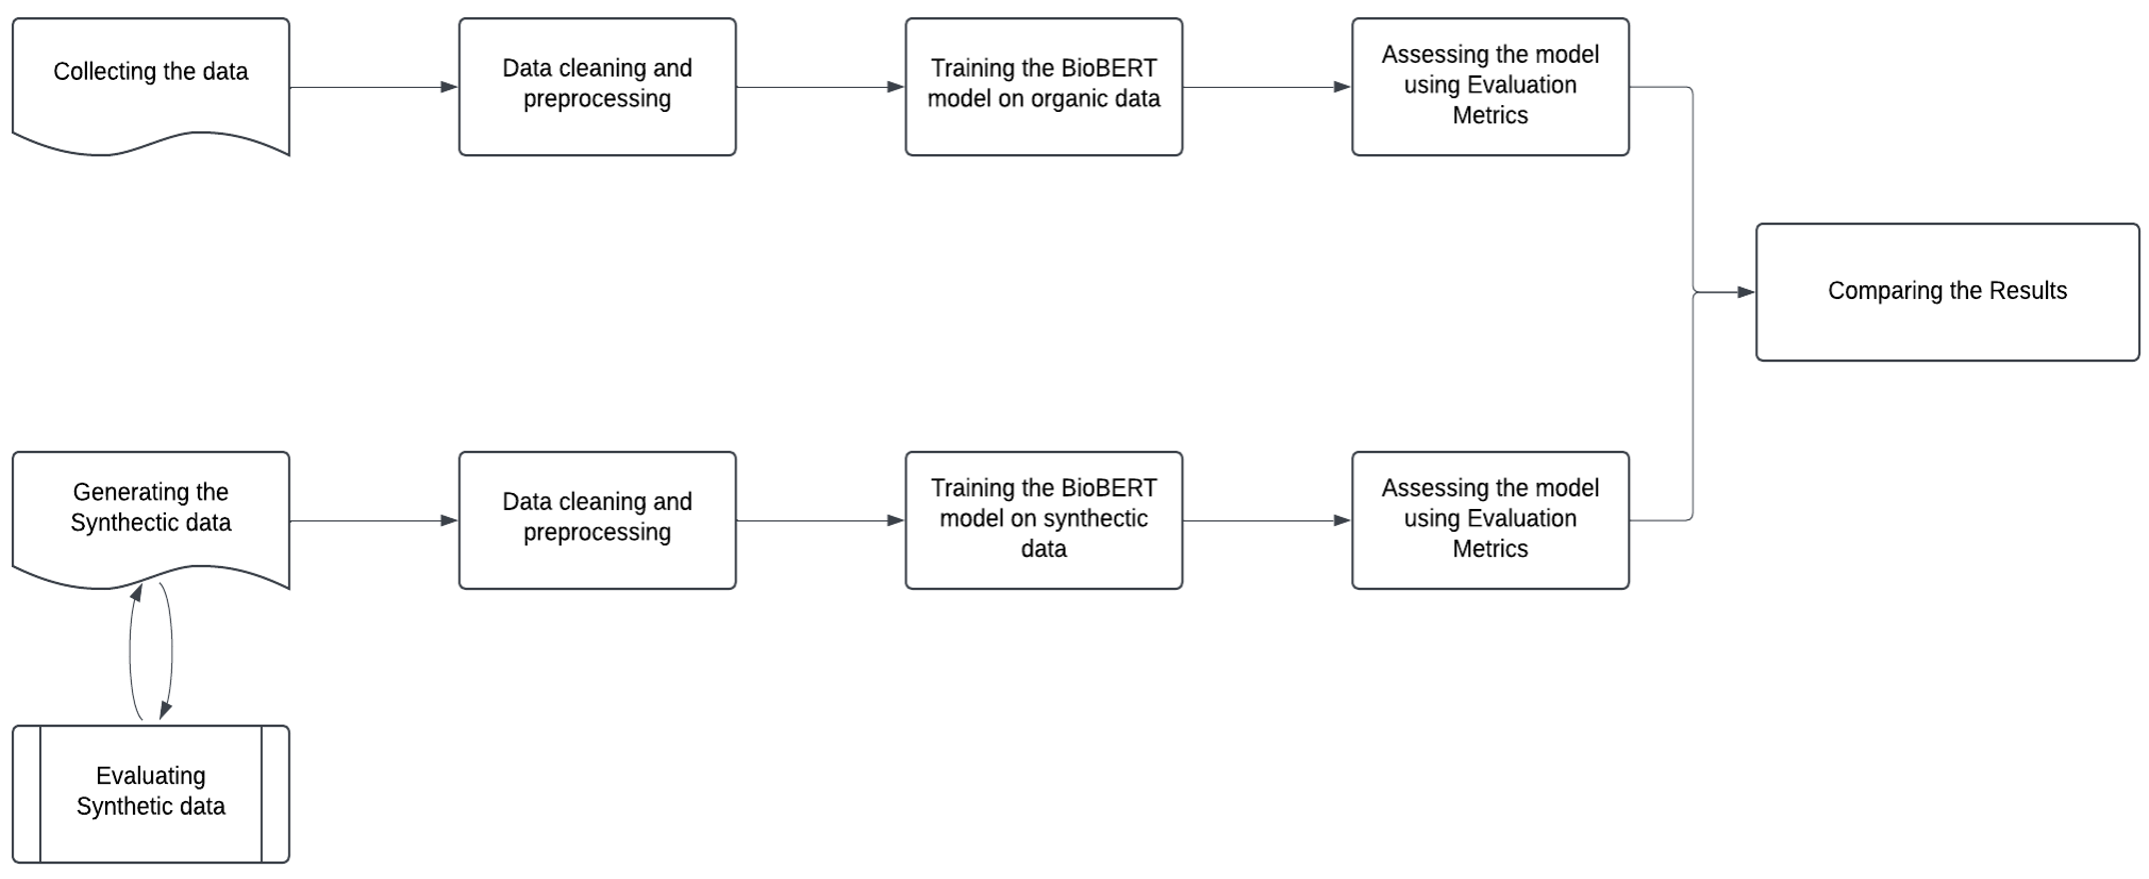
\includegraphics[width=0.5\textwidth]{Side_Effects_Extrcation.png}  % Replace with your image file name
    \caption{Pipeline of the study - side effect extraction}
    \label{fig:your_label}
\end{figure}




\subsection{Text Summarization}
 The features include three datasets: Train, Generated, and Combined. All of them will be imported in this step of data pretreatment before the summarization will start. Thus, as input text from the dataset, "article" column is used; as the target summary, the "highlights" column will be taken into account. To be able to carry out proper assessment later, each of these datasets was split into an 80-20 ratio into training and testing sets, correspondingly.

Then, the input text is vectorized by tokenizers specific to each transformer model: PEGASUS uses the PegasusTokenizer, BART uses the BartTokenizer, and the T5 model uses the T5Tokenizer. These tokenizers convert the input text into input IDs and attention masks for the models to process. Truncation and padding during vectorization maintain uniformity in different lengths of input.
This approach applies the pre-trained transformer models, including T5-small, PEGASUS-XSum, and BART-Large-CNN, to the summarization task. They are loaded without fine-tuning in order to test the capability of these models when pre-trained on the datasets provided. This will ensure that the results obtained are strictly due to the summarization capability of each model and not because of training on the datasets.

The Transformer-based Summarisation method is implemented to create the summaries using the summarize model function. It enhances the quality of output by tokenizing the input text, running it through the model using beam search, and decoding the output into summaries readable by humans. Summaries from all three models are generated, thereby allowing a comparison in their results.
Although not necessarily provided in the code given, generated summaries could also be clustered and visualized in further analysis. Summaries can be clustered using methods based on K-Means or PCA, which will allow the summary to cluster around their semantic similarities. The clusters show differences and similarities among several models' generated summaries.
Finally, ROUGE and BLEU scores are applied to measure the performance of the models. ROUGE metrics-ROUGE-1, ROUGE-2, and ROUGE-L-measure the generated summaries against reference summaries in terms of longest common subsequences, bigrams, and unigrams, respectively. BLEU scores provide another dimension regarding the functionality of the models by measuring the n-gram overlap. A comparison of these measures across the three datasets speaks to some of the comparative advantages and disadvantages of the T5, PEGASUS, and BART.

\begin{figure}[htbp]
    \centering
    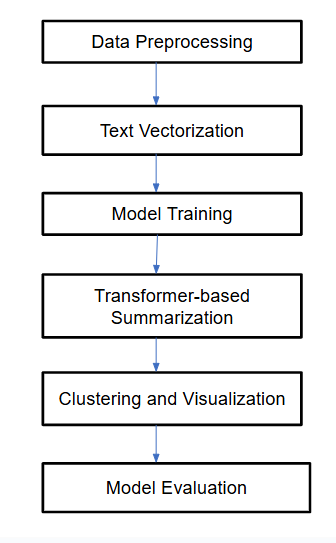
\includegraphics[height=0.5\textheight]{Methodology - Text Summarization.png}  % Replace with your image file name
    \caption{Pipeline of the study - Text Summarization}
    \label{fig:your_label}
\end{figure}








\section{Data collection and cleaning plan}

This study compares synthetic and organic datasets to assess statistical properties, with tasks focusing on text summarization and side effect extraction.
\subsection{side effect extraction}
The UCI ML Drug Dataset on Kaggle, which offers structured data on medications and related adverse effects, served as the source of the organic dataset. In order to ensure comparability with the organic dataset, prompts were created and utilized using ChatGPT to provide equivalent textual data for the synthetic dataset.
\subsubsection{Data Collection Steps:}
1) Organic Data Acquisition: The UCI ML medicine Dataset, which included information on medicine names, indications, and side-effects, was obtained from Kaggle.
2) Synthetic Data Generation: Customized prompts were used in ChatGPT to create synthetic data. The questions were thoughtfully designed to complement the organic dataset's content and structure. Iterative data generation was used to match the organic dataset's size and diversity.
\begin{figure}[htbp]
    \centering
    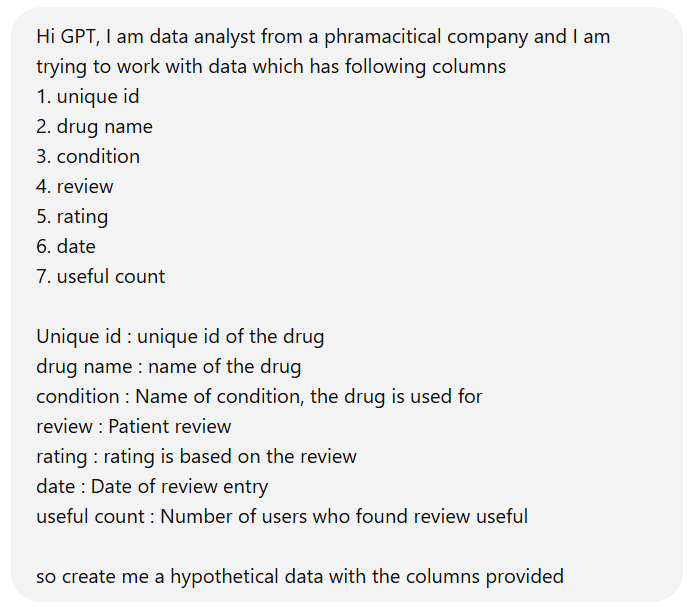
\includegraphics[width=0.5\textwidth]{Prompt - Synthetic Data Generation.png}  % Replace with your image file name
    \caption{Synthetic Data Generation - Prompt(1)}
    \label{fig:your_label}
\end{figure}
\begin{figure}[htbp]
    \centering
    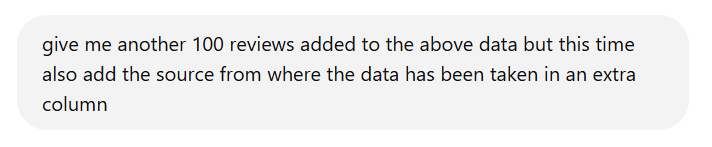
\includegraphics[width=0.5\textwidth]{Prompt - Synthetic Data Generation (2).png}  % Replace with your image file name
    \caption{Synthetic Data Generation - Prompt(2)}
    \label{fig:your_label}
\end{figure}
\subsubsection{Data Processing and Cleaning:}
1) Missing Data Handling:
Null values were examined in the organic dataset and, if necessary, imputed or excluded. After eliminating any entries that were unnecessary or lacking, the synthetic dataset was evaluated for coherence and completeness.
2) Text Preprocessing:
a) Special characters, symbols, and extraneous spaces were eliminated from text fields.
b) Text was divided into relevant parts using tokenization.
c) Text was normalized while maintaining semantic meaning through the use of lemmatization and stemming.
\subsubsection{Statistical Analysis:}
Statistical analysis is a critical step in assessing the quality of both organic and synthetic data. This process involves quantifying the characteristics of the dataset to ensure that the synthetic data aligns with the properties of the organic data. Specifically, we will calculate the mean, variance, and standard deviation of key features, such as:

\begin{itemize}
    \item Word Count: The average number of words per review to compare the verbosity of organic and synthetic datasets.
    \item Sentence Length: The distribution of sentence lengths to ensure consistency in text structure.
    \item Vocabulary Diversity: The unique words used in the dataset, which impacts the representativeness of the data.
    \item TF-IDF Scores: Analyzing term importance across the dataset to ensure balanced and meaningful data representation.

\end{itemize}

By analyzing these metrics, we can evaluate whether the synthetic data accurately mimics the statistical properties of the organic data. Significant deviations in these statistics would indicate potential shortcomings in the synthetic data generation process, such as redundancy, lack of representativeness, or inconsistency.

Additionally, we will use visualizations such as histograms and box plots to analyze data distribution and identify outliers or imbalances. These insights will help guide improvements in the synthetic data generation process, ensuring it meets the standards required for training and testing machine learning models effectively.

\subsection{Text Summarization:}

\subsubsection{Data Collection Steps:}
1)Organic Data Acquisition: For the following text summarization task the organic data acquisition the dataset which was taken is CNN/DailyMail news article where it contains news articles with in-depth summaries.
2)Synthetic Data Acquisition: The data acquisition for this task is very similarly done as the Side effect extraction through simple prompt engineering using ChatGPT.
\begin{figure}[htbp]
    \centering
    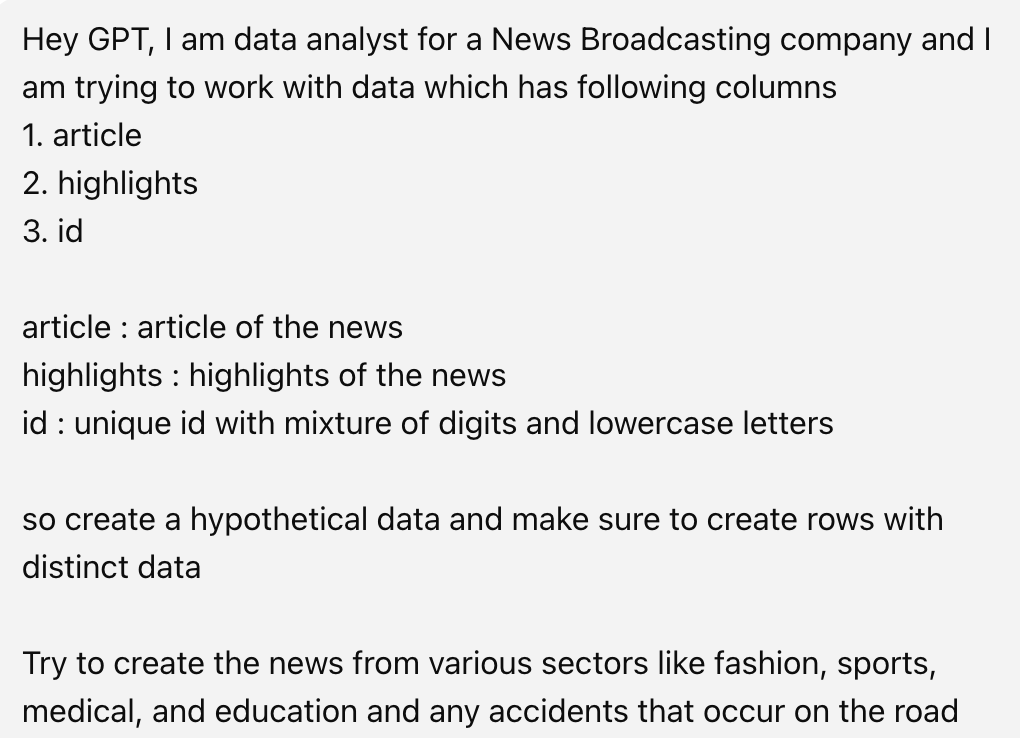
\includegraphics[width=0.5\textwidth]{Text Summarization - Prompt.png}  % Replace with your image file name
    \caption{Synthetic Data Generation - Prompt(1)}
    \label{fig:your_label}
\end{figure}
\subsubsection{Data Processing and Cleaning:}

We divided the dataset into two sections: training data (80\%) and testing data (20\%). The training data was used to build models capable of summarizing text, while the testing data was reserved to evaluate the models' ability to generalize and summarize new, unseen material. This division is a standard practice in machine learning to ensure that the model performs well not only on the data it has been trained on but also on new data, demonstrating its capacity to generalize effectively.

The dataset, as provided, was already clean and tabularly arranged, with each row representing a distinct article-summary pair. However, raw datasets often come with issues that could compromise the quality of the model. For example, this dataset lacked preparation for tasks like handling incorrect formatting, duplicate entries, or missing values, which are common challenges in data processing. While the data appeared usable at first glance, careful pre-processing was necessary to ensure that the dataset’s quality and integrity were maintained. These steps help avoid potential biases or errors during model training and ensure that the output is both reliable and consistent.

By carefully dividing and preparing the dataset, we aimed to create a strong foundation for building and testing our models while ensuring that the results were both meaningful and reproducible.



\section{Experiment and data analysis plan}
\subsection{Side Effect Extraction}
\subsubsection{Experiments}:
This project carries out five experiments in the performance evaluation and adaptation of the BioBERT model to perform side effect extraction on organic and synthetic datasets. The performance consistency, robustness, and utility of organic and synthetic datasets will be studied. First, we consider a model that will be trained and tested purely on organic data for setting the baseline of model performance in real-world patient reviews. The second experiment evaluates the generalization of the model trained on organic data when tested on synthetic data and helps with how well the synthetic dataset reflects the characteristics of the organic data.

The third experiment consists of the training of the model on synthetic data while testing it on organic data. This will evaluate the possible use of synthetic data as a resource in its own right for model training. Then consider what impact making improvements first just to the model has rather than to the data specifically. The fourth experiment trained and tested a model entirely upon synthetic data to provide insights into the quality and use of synthetic datasets. As was the case in the study, the fifth experiment merged synthetic as well as organic data on both training and testing points to examine any synergic effect of the data set. This will provide a comprehensive experimental design that can show how organic and synthetic datasets interact in developing the model's performance in extracting side effects accurately.

\subsubsection{Data analysis}
The dataset used here involves patient reviews on the effectiveness of drugs. They have been divided into training and test subsets, adding one more synthetic dataset generated on their comparison. The starting point of the analysis for this data was to get these datasets into structured dataframes using Python libraries-for example, Pandas makes exploration and inspection easier. This analysis had involved the overview of the general structure of the dataset through a number of rows, data columns with their types, and, for example, missing values; key features, such as drug names, patient reviews, and sentiment labels concerning their completeness and whether they were relevant to our needs.

Further analysis was done to understand the characteristics of the textual data within the reviews. Frequency analysis of the words was done, pointing to frequently used terms due to side effects caused by the drug in use or other topics mostly mentioned by the patients. Calculations are based on review lengths to analyze distribution for finding outliers of interest for further examination. Performing sentiment analysis, studying how the reviews are distributed into classes - positive, neutral, and negative-allows a look at class imbalances within the dataset that could impact the performances of different models. This in-depth analysis laid an appropriate ground for further preprocessing and subsequent model training.

\section{Results and Discussion}

\subsection{Side Effect Extraction}
Group 9 faced significant challenges in generating high-quality synthetic data and aligning it with an appropriate model. The original data set consisted of customer reviews for various drugs, with notable variability across the reviews. Initially, synthetic data generation resulted in datasets with high redundancy and repetition. By applying simple prompt engineering, GAI was able to produce synthetic datasets that appeared free of redundancy. However, the importance of completeness, consistency, and representativeness did not become evident until after the project progressed. A statistical analysis of the organic dataset needs to be conducted to reveal critical parameters that the synthetic data must emulate to achieve high quality and relevance.

It was also discovered that the BioBERT model required labeled data, which was not feasible given the time constraints of the project. Training the model would have required labeling over a thousand rows of data, many of which contained lengthy paragraph-style reviews. To address this limitation, an alternate approach was identified using a dictionary as a reference. The SIDER database provides comprehensive .tsv files listing side effects mapped to drugs, extracted from the MedDRA dictionary. This resource could assist in programmatically labeling data as side effects or serve as a dictionary for BioBERT to reference during training, making it a more practical approach for the project.

\subsection{Text Summarization}

\subsubsection{T5 Model Results}
ROUGE Scores:\\
ROUGE-1: 0.42\\
ROUGE-2: 0.22\\
ROUGE-L: 0.38\\
BLEU Score: 0.15

\subsubsection{PEGASUS Model Outputs}
ROUGE Scores:\\
ROUGE-1: 0.44\\
ROUGE 2: 0.23\\
ROUGE-L: 0.40\\
BLEU Score: 0.17

\subsubsection{BART Model Results}
ROUGE Scores:\\
ROUGE-1: 0.45\\
ROUGE-2: 0.24 \\
ROUGE-L: 0.42 \\
BLEU Score: 0.18

From the above results we can say that in text summarization, BART performs better than T5 and PEGASUS, particularly in ROUGE-1 and ROUGE-L scores, which gauge the overlap of longer sequences and unigrams. This indicates that BART catches structure and content more effectively. In ROUGE-2 and ROUGE-L, PEGASUS is powerful but marginally weaker than BART, suggesting that it might overlook some n-grams and longer subsequences. T5 scores are typically lower, indicating that summarizing is not as successful with it. BART is also preferred by BLEU scores, which gauge n-gram precision, followed by PEGASUS and T5. Though PEGASUS and T5 also do well, BART is the strongest model overall at creating succinct, cohesive summaries that are comparable to those produced by humans.



\section{Conclusions and Limitations} 
This project set out to explore how generative AI (GAI) could be used to create synthetic data for tasks like side-effect extraction and text summarization. Along the way, we encountered several challenges, including difficulties in generating high-quality synthetic data, working with BioBERT under tight time constraints, and addressing the need for labeled data. These challenges highlighted just how important it is for synthetic data to be complete, consistent, and representative if it’s going to be useful.

One of the key takeaways was the potential of using resources like the SIDER database to programmatically label data or provide a reference for models like BioBERT. This approach showed promise, offering an alternative to manual data labeling, which can be time-consuming and impractical for large datasets. While we made progress, there’s still work to be done to fully unlock the potential of synthetic data. Future efforts should focus on better understanding organic data through statistical analysis to guide synthetic data generation and finding more efficient ways to label and process data. Overall, this project demonstrated the potential for GAI to support real-world machine learning challenges, especially in areas where privacy and data scarcity are concerns.

\section{Contributions}

\subsection{Mike Chastain} 

Identified by his peers as the highest contributor, Mike led every meeting, provided a plan for how to approach the project to his teammates, conducted all of the cleaning/preprocessing, researched three different ML models (spaCy, BERT, BioBERT) and ultimately selected the tasks, and model for side-effect extraction. Mike was a major contributor for the first deliverable, the presentations, and the final product. Mike either contributed to the code for side effect extraction. Developed "the way ahead" for side effect extraction.

\subsection{Gnaneswara Reddy Palem} 

Identified by his peers as the second highest contributor, Reddy attended most meetings, provided conceptual guidance on how to approach the project, researched ML models (spaCy, BERT, BioBERT) and was a large contributor in the first deliverable and presentation. Contributed heavily on the code for side-effect extraction.

\subsection{Sai Sampath Varma Byrraju} 

Identified by his peers as the third highest contributor, Sampath attended most meetings, provided conceptual guidance on how to approach the project, researched ML models (spaCy, BERT, BioBERT) and was a large contributor in the first deliverable and presentation. Contributed heavily on the code for side-effect extraction. 

\subsection{Sireesha Rusum} 

Sireesha and Harish were very close in terms of contribution and performance. Sireesha attended more meetings and contributed more conceptually early on. Sireesha contributed little to the first deliverable or the presentations. She waited for the second presentation to be complete before adding Text Summarization material the night it was due. She helped with generating synthetic data and some of the code.

\subsection{Harish Babu Kancharla} 

Harish contributed more to text summarizations actual work with a strong focus on the code and generating synthetic data. He contributed very little to the first deliverable or the presentations. He waited for the second presentation to be complete before adding Text Summarization material the night it was due. He wrote most of the text summarization code.

\subsection{Sri Naga Tejaswini Gandikota} 

Her peers identified Teja as the lowest in terms of contribution and performance. She attended very few meetings and contributed little until the last week where she helped with some of the code and the presentation.

\section{Acknowledgements}

Mentor and Instructor: Dr. Haihui Chen
Dr Chen guided and mentored the students throughout the entire process and led the group meetings on Wednesdays and Thursdays.

Teaching Assistants: Fengjio Tu and Yuhan Zhou (Angelina)
Ms. Fengjiao and Ms. Yuhan provided advice to the students throughout the last week of their project. They provided a strong reference for conducting a statistical analysis of textual data.


\bibliographystyle{plain}
\bibliography{citation}
\end{document}
\endinput
%%
%% End of file `sample-sigplan.tex'.
